流域人水系统是典型的社会-生态系统,系统演变机制是社会-生态系统研究的核心内容。
根据侧重点的不同,武旭通将当前社会-生态系统互馈的机制总结为“时”(系统弹性)、“空”(全程耦合)、“构”(结构匹配)、“阈”(地球界限)四个方面,其中“时”为包含弹性和稳态转换在内的一组概念,是研究社会-生态系统动态演化的重要理论框架\cite{WuXuTong2021},对理解人水系统的演变机制至关重要。
本节综述了与稳态转换密切相关的核心概念,并分别围绕“驱动因素、表现特征、级联效应”者三个稳态转换的核心要素,总结了分析人水系统演变机制的主要路径。

\subsubsection*{稳态转换与相关概念}

% 宋嘉熙 的 地理学报
韧性(Resilience)是处于动态平稳的社会-生态系统面对变化时通过缓冲、适应或转变等方式响应以维持人类福祉的能力[30],稳态转换(Regime shifts)指系统的结构和功能发生大规模重组并突破这种平稳状态的过程[6–9],在生态系统[10–12]、气候系统[13–16]、经济系统[17–19]、及其它复杂系统[20,21]中均可能发生,具有不易预测、难恢复的特点[7,22,23]。
社会-生态系统研究中通常使用“球-杯模型”描述稳态转换:不同稳态就像系统状态空间中凹陷的“杯子”,将系统实际状态则如同在不同凹陷间滚动的“小球”,状态空间的变化(参数驱动)或小球受到外力(外力驱动)时都可能推动系统状态在不同稳态间发生转换[8,36](图\ref{ch2:fig:regime_shift})。
参量驱动是当外界条件(环境参数)发生变化时削弱系统韧性被诱发稳态转换[7,8],变量驱动则是系统内部或外部变量推动系统突破阈值所触发的稳态转换,(图\ref{ch2:fig:regime_shift})。
除了驱动因素外,系统稳态转换的发生可能致使系统功能与产出(Outcome)发生变化,或进一步触发其它的级联效应(Effect)。
识别稳态转换应从驱动力、现象、与效应(Effects)这三个稳态转换的核心要素切入,厘清系统间反馈机理、分析关键要素间交互作用,揭示社会-生态系统稳态转换的成因类型、现象特征与产出/外溢效应。

% Description of system regime shift by ball-cup model and fold bifurcation
\begin{figure}[htb] % use float package if you want it here
    \centering
    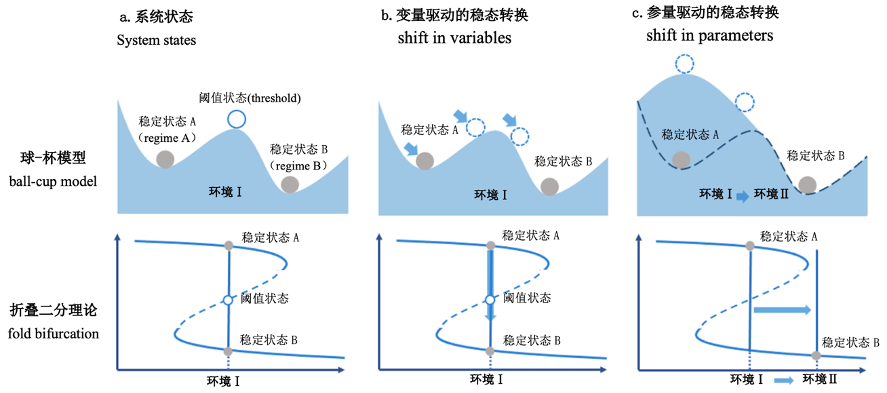
\includegraphics[width=\textwidth]{img/ch2/ch2_regime_shift.png}
    \caption[球-杯模型和折叠分岔理论对系统稳态转换的描述]{球-杯模型和折叠分岔理论对系统稳态转换的描述。
    假设系统中最多可能有2个稳定平衡状态,即稳定状态A(regime A)和稳定状态B(regime B)和阈值(threshold):
    a)环境Ⅰ条件下,球-杯模型(ball-cup model)和折叠二分理论(fold bifurcation)对系统各种状态的表征。
    b)系统稳态转换过程。变量驱动的稳态转换(shift in variables):环境Ⅰ不变时,处于稳定状态A的系统在干扰下自身突破阈值状态转换为稳定状态B。
    c)参量驱动的稳态转换(shift in parameters)。环境Ⅰ变为Ⅱ,迫使处于稳定平衡状态A的系统向新环境下仅存的稳定平衡状态B转换。(改自文献[7],[8])}\label{ch2:fig:regime_shift}
\end{figure}

\subsubsection*{稳态转换的驱动因素}

Rocha等人发现不断累积的人为干扰压力和气候变化是最常见的两类稳态转换驱动因素,无论以变量还是参量的形式出现[60,61]。
Ji等根据水-沙调节方案和河口河道迁移两个主要驱动因素变化的时间节点,结合不同阶段河口侵蚀-沉积量与河口排沙量确定了河口侵蚀-积聚模式的稳态转换过程[84]。
Bao等分析黄河中游水平衡系统稳态转换时,识别出气候驱动因素和土地利用/覆盖显著变化的阶段,通过验证不同阶段水平衡状态的差异确定了不同稳态阶段后,进一步定量解析了驱动水平衡状态转换的具体机制[85]。
此类分析路径的关键在于准确选择系统驱动力的定量表征,因此需要预设系统稳定状态和驱动力之间的关系,多用于驱动力易于识别的干扰因素,如持续减少的林地、持续周期性变化的气候等。

另一类常见人为干扰是水治理措施,单独某个治理举措对系统稳态产生的驱动力及其作用方向通常是复杂多变的,“稳态循环”理论有助于理解这类驱动力触发的稳态转换。
该理论指出系统在不同尺度下可自组织历经适应性循环的“开发”(Growth)、“保护”(Senescence)、“释放”(Collapse)、“更新”(Renewal)四个阶段[63],也有学者总结为“涌现”(Emergence)、“制度化”(Institution)、“更新”(Renewal)三阶段(Chaffin and Gunderson, 2016)。
根据“主动改变不良的社会-生态系统状态”与“调节并维持良好的社会-生态系统状态”两种不同的目的,这种系统内自组织形成的治理措施可分为自上而下的“转型治理”和自下而上的“协作治理”两类。
转型治理关注社会-生态系统社会-生态系统的释放和更新阶段,强调适应性治理的实现,以及主动促使社会-生态系统完成状态的更新[64];协作治理则强调适应性治理制度化过程,旨在通过利益相关者间自组织的协作模式来实现社会-生态系统的开发与保护[65]。
无论自上而下或自下而上,流域治理既可能是维持稳态的原因,也可能成为稳态转换的触发因素,需在分析治理措施的作用机制时加以甄别。

\begin{figure}[htb] % use float package if you want it here
    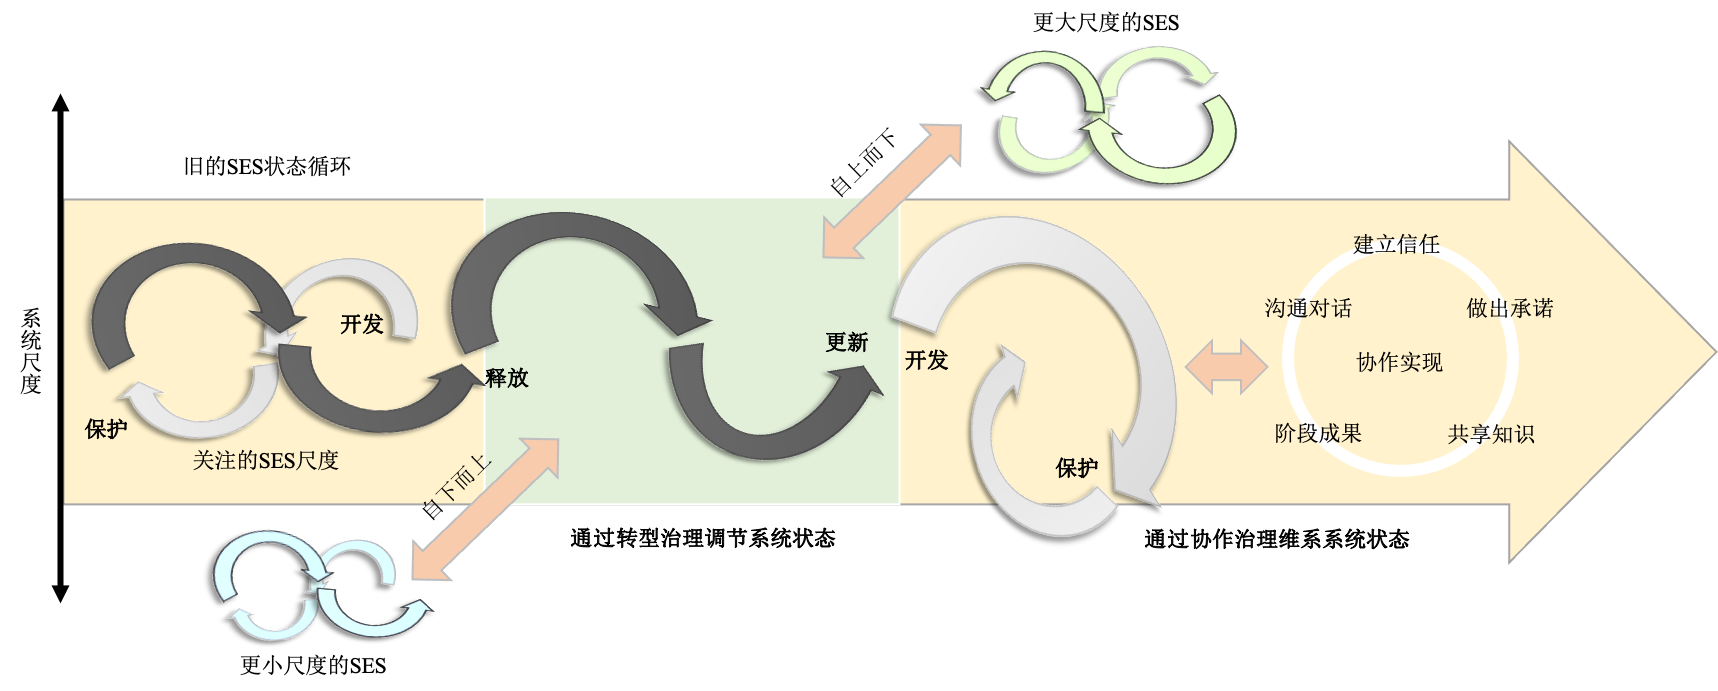
\includegraphics[width=\textwidth]{img/ch1/ch1_governance_driver.png}
    \caption[社会-生态系统状态循环]{社会-生态系统状态循环与转型治理、协作治理的关系
    Fig.4  The relationship between social-ecological system adaptive cycle and transition / collaborative governance
    SES状态循环包括:开发阶段$r$,保护阶段$K$,释放阶段$\varOmega$,更新阶段$\alpha$;图中展示旧的SES因转型治理而进入新的状态循环,并因协作治理的实现而延长开发保护阶段的过程;转型治理可受其它尺度SES的影响[64,66];协作治理的主要实现过程包括F-F-D(Face to Face Dialogue, 当面沟通),T-B(Trust-Building, 建立信任),C-P(Commitment to Process, 过程承诺),S-U(Shared Understanding, 信息对称),I-O(Intermediate Outcomes, 阶段成果)五步骤的循环[65,68,58]。}\label{ch1:fig:governance_driver}
\end{figure}

\subsubsection*{稳态转换的表现特征}

聚焦于稳态转换过程中所表征出的现象是分析稳态转换最常见的路径,通过寻找合适的指标识别系统互馈变量或相关解释变量的趋势突变,检测稳态转换现象。
一旦可获得高质量时间序列数据,相关的检测方法非常丰富,常见的包括趋势分析、断点检测或断点回归等。
Wang等利用t检验的循序算法(sequential t-test analysis of the regime shifts ,STARS)和加性季节和趋势断点(Breaks For additive Season and Trend, BFAST)模型两种方法检测$1950 \sim 2011$年黄河流域上中下游径流和输沙量的突变时间点以确定稳态转换时期[64];
Zhao等利用曼-肯德尔(Mann-Kenall)趋势分析法和加性季节和趋势断点检测模型识别出1921—2011年期间黄河月径流量趋势突变,重建天然径流量,量化人类活动对流量稳态转换的影响程度[82]。

在识别稳态转换现象的基础上,还可以进一步将其与稳态转换驱动力相关联。
Yang等利用 Pettitt 检验计算稳态转换指数(Regime Shift Index, RSI),探测海流兔河$1957 \sim 2007$年间径流的稳态转换,并与气候和土地利用变量的突变点对比分析,证实土地利用政策驱动了径流的稳态转换[49]。
Niu等检测了黄河三角洲系统降水量,温度,月径流量和归一化植被指数(Normalized Difference Vegetation Index,NDVI)等多个现象相关变量共同的分解趋势断点,识别水文气候-植被系统的稳态转换时期,分析各阶段内气候水文变量与NDVI间产出效应[83]。
聚焦稳态转换的现象表征,易于直观划分稳态转换的时期探,且有着成熟的数据检测技术;但如果忽略对驱动和效应的结合分析,容易对稳态转换的驱动-响应机制表达不够全面。

\subsubsection*{稳态转换的级联效应}

级联效应是系统稳态转换发生后产生的一系列后续影响,以此切入分析能应对系统内互馈关系复杂的情况,根据受到级联效应影响的要素在系统内或系统外又可分为内联效应和外溢效应。
Sun等对黄河中游对泥沙运输稳态转换机制展开研究时,利用沉积率曲线的参数变化刻画出泥沙运输稳态转换的产出效应变化特征,并解释了生态恢复对泥沙运输稳态的调节作用[50]。
Wu等面对互馈关系复杂的黄土高原社会-生态系统稳态转换时,利用各阶段人口数量、耕地面积和森林覆盖率三个变量间的回归参数量化社会-生态系统内部要素交互作用的稳定状态,借助社会-生态要素间相互关系的组合来识别稳态转换的发生阶段,揭示稳态转换不同阶段系统关系变化和外溢效应\cite{wu2020a}。
Kidder等对古代堤坝建设触发黄河河道泥沙淤积系统稳态转换展开研究时,利用外溢系统中黄河下游洪水的频率和规模变化确定稳态转换发生时期,并证实堤坝作为驱动因素对泥沙淤积存在着强烈正反馈[86]。
由于有助于识别复杂的社会-生态系统稳态转换的发生机制,此类分析路径正成为稳态转换实证研究的热点,但需要准确选择与系统反馈过程联系紧密的级联现象,因此也需要关于系统稳态的先验知识。

综上所述,尽管已有研究从驱动因素、表现特征、级联效应三个不同的要素出发不断发展人水系统的稳态转换机制分析,相应的量化方法也在不断丰富。
但是,稳态转换作为大规模的系统重组,流域人水关系变化应伴随多要素的同步转变,仅从单一要素出发的研究仍易导致对其机制认识不全面,目前仍缺乏系统整合“驱动-现象-效应”的多要素分析。
